\documentclass[t]{beamer}

\usepackage{etex}
%\documentclass[notes,t]{beamer}

\setbeamertemplate{bibliography item}[text] %default is an icon of an

%\usepackage{mathchars}
\usepackage{amsmath}
\usepackage{mathtools}

\usepackage{booktabs}
\usepackage{float}              %for forcefully placing diagrams 
\usepackage{subcaption}

\usepackage{algorithm}
\usepackage{algpseudocode}
\newcommand{\tab}[1]{\hspace{.08\textwidth}{#1}} % indent tab for data
                                                  % structs in algos
 \newcommand{\LineIf}[3]{ {#1}
   \algorithmicif\ {#2}
   \algorithmicelse\ {#3} } % inline X if Y else Z

\definecolor{oblack}{HTML}{0D1B2E}
\definecolor{deepblue}{HTML}{183152}
\definecolor{navyblue}{HTML}{375D81}
\definecolor{bluegreen}{HTML}{ABC8E2}
\definecolor{beige}{HTML}{C4D7ED}
\definecolor{cream}{HTML}{E1E6FA}
\definecolor{owhite}{HTML}{F9FFFF}
\definecolor{redi}{HTML}{A5121E}
\definecolor{greeni}{HTML}{3E700F}

\definecolor{col2}{HTML}{ABC8E2}
\definecolor{col1}{HTML}{E1E6FA}
\definecolor{col3}{HTML}{F0EAB3}
\definecolor{col4}{HTML}{375D81}
\definecolor{col5}{HTML}{C4D7ED}


\newcommand{\hilight}[1]{\colorbox{bluegreen}{#1}}

\setbeamercolor{normal text}{fg=oblack}
\setbeamercolor{alerted text}{fg=redi}
\setbeamercolor{background canvas}{bg=owhite}
%\setbeamercolor{block body alerted}{bg=normal text.bg!90!black}
%\setbeamercolor{block body}{bg=normal text.bg!90!black}
%\setbeamercolor{block body example}{bg=normal text.bg!90!black}
%\setbeamercolor{block title alerted}{use={normal text,alerted text},fg=alerted text.fg!75!normal text.fg,bg=normal text.bg!75!black}
\setbeamercolor{block title}{fg=deepblue}
%\setbeamercolor{block title example}{use={normal text,example text},fg=example text.fg!75!normal text.fg,bg=normal text.bg!75!black}
%\setbeamercolor{fine separation line}{}
\setbeamercolor{frametitle}{fg=navyblue}
%\setbeamercolor{item projected}{fg=black}
%\setbeamercolor{normal text}{bg=black,fg=yellow}
%\setbeamercolor{palette sidebar primary}{use=normal text,fg=normal text.fg}
%\setbeamercolor{palette sidebar quaternary}{use=structure,fg=structure.fg}
%\setbeamercolor{palette sidebar secondary}{use=structure,fg=structure.fg}
%\setbeamercolor{palette sidebar tertiary}{use=normal text,fg=normal text.fg}
\setbeamercolor{section in sidebar}{fg=beige}
\setbeamercolor{section in sidebar shaded}{fg=cream}
%\setbeamercolor{separation line}{}
\setbeamercolor{sidebar}{bg=deepblue}
\setbeamercolor{sidebar left}{bg=deepblue}
\setbeamercolor{author in sidebar}{fg=owhite}
\setbeamercolor{title in sidebar}{fg=owhite}
%\setbeamercolor{sidebar}{parent=palette primary}
%\setbeamercolor{structure}{bg=black, fg=green}
\setbeamercolor{subsection in sidebar}{fg=owhite}
\setbeamercolor{subsection in sidebar shaded}{fg=owhite}
\setbeamercolor{title}{fg=deepblue}
\setbeamercolor{titlelike}{fg=deepblue}
\setbeamercolor{section in toc}{fg=navyblue}
\setbeamercolor{subsection in toc}{fg=bluegreen}
\setbeamercolor{section number projected}{bg=navyblue,fg=cream}
\setbeamercolor{itemize item}{fg=navyblue}
\setbeamercolor{block title alerted}{fg=redi}
\setbeamercolor{block title example}{fg=greeni}
\setbeamercolor{figure caption name}{fg=redi}
\setbeamercolor{figure caption}{fg=redi}
\setbeamercolor{description item}{bg=deepblue,fg=deepblue}

\captionsetup[figure]{labelfont={color=redi,footnotesize},textfont={footnotesize,color=oblack}}

\usepackage{pgfplots}
\usepackage{tikz}
\usetikzlibrary{shapes,
  arrows,
  chains,
  matrix,
  positioning,
  fit,
  scopes,
  calc,
  decorations.pathmorphing}
\makeatletter
\tikzset{join/.code=\tikzset{after node path={%
\ifx\tikzchainprevious\pgfutil@empty\else(\tikzchainprevious)%
edge[every join]#1(\tikzchaincurrent)\fi}}}
\makeatother
\tikzset{>=stealth',every on chain/.append style={join},
         every join/.style={->},
         snake it/.style={decorate, decoration=snake}}
\tikzstyle{labeled}=[execute at begin node=$\scriptstyle,
   execute at end node=$]

\AtBeginSection[]
{
  \begin{frame}
    \tableofcontents[currentsection]
  \end{frame}
}

\def \mheight {0.5cm}
\def \mwidth {0.5cm}

\tikzstyle{bx}=[
  fill, 
  minimum height=\mheight, 
  minimum width=\mwidth, 
  shape border rotate=90, 
  shape aspect=0.1,
  rounded corners=2mm
]

\tikzstyle{cld}=[
  cloud, 
  cloud puffs=15.7, 
  cloud ignores aspect, 
  minimum height=\mheight,
  minimum width=\mwidth, 
  align=center
]

\tikzstyle{dtb}=[
  fill,
  chamfered rectangle,
  chamfered rectangle xsep=2cm,
  minimum height=\mheight, 
  minimum width=\mwidth,
  rounded corners=1mm
]

\usepackage[utf8]{inputenc}
\usetheme{Hannover}
\usecolortheme{dolphin}

\begin{document}

\title[Analysis of Wikipedia hitories] % (optional, only for long titles)
{Automatically defining collaborative share through
    the automatic, na\"ive string analysis of Wikipedia article
    revision histories}
\author % (optional, for multiple authors)
{W~Marsey}
\institute{Imperial College London} % (optional)
\date % (optional)
{Sep 2014}
\subject{Computing Science}

\frame{\titlepage}

\section{Introduction}
  %%%%%%%%%%%%%%%%%%%%%%%%%%%%%%%%%%%%%%%%%%%%%%%%%%
  %%%%%%%%%%%%%%%%%%%%%%%%%%%%%%%%%%%%%%%%%%%%%%%%%%
  %%%%% 
  %%%%% INTRODUCTION
  %%%%%
  %%%%%%%%%%%%%%%%%%%%%%%%%%%%%%%%%%%%%%%%%%%%%%%%%%
  %%%%%%%%%%%%%%%%%%%%%%%%%%%%%%%%%%%%%%%%%%%%%%%%%%

\begin{frame}{Why?}
  \begin{itemize}[<+->]
  \item Interesting because automated collaboration is only becoming
    more popular.
  \item How do we define authorship in this context?
  \item Wikipedia is a good model data source because its free,
    public, simple.
  \end{itemize} 
  \only<4>{

    We investigate how we may define share on Wikipedia. As a simple
    model for more proprietary work. 

  }
\end{frame}

\begin{frame}{Past studies}
  On Wikipedia:
  \begin{itemize}[<+->]
  \item Wide array of past studies.
  \item Tangential studies concentrate on `quality'.
  \item Last year's paper looks comparison's between texts.
  \end{itemize} 

  \onslide<4->{

    We are going to look at how we:
    \begin{itemize}
      \item Automate, improve \& expand on last year's work
      \item Change our idea of what makes a good edit
      \item Introduce a better approach
    \end{itemize}
  }

\end{frame}
  %%%%%%%%%%%%%%%%%%%%%%%%%%%%%%%%%%%%%%%%%%%%%%%%%%
  %%%%% COPYRIGHT
  %%%%%%%%%%%%%%%%%%%%%%%%%%%%%%%%%%%%%%%%%%%%%%%%%%
  \begin{frame}[shrink]
    \setbeamercovered{transparent}

    \frametitle{On copyright} 
    \framesubtitle{What does existing legislature say?}
    
    \begin{itemize}[<+->]
      \item Joint works are inseparable, made with intent
      \item Ownership is complex / changeable
      \item Share is divided according to licensing arrangements
    \end{itemize}    
    
    \only<1>{
      
      \begin{quote} When two or more authors prepare a work
        with the intent to combine their contributions into
        inseparable or interdependent parts, the work is considered
        joint work and the authors are considered joint copyright
        owners. (UK Intellectual Property
        Office) \cite{what-joint-authorship}
      \end{quote}

    }
    
    \only<1>{

      \begin{quote} Where two or more people have created a
        single work protected by copyright and the contribution of
        each author is not distinct from that of the
        other(s).(Stanford: Copyright \& Fair
        Use) \cite{joint-authorship}
      \end{quote}

    }

    \only<2>{

      \begin{quote}
        ownership of copyright can be transferred, so where something
        is produced that has involved contributions from more than one
        person, it would be possible for copyright in all the material
        to be owned by one person as a result of appropriate
        transfers. Indeed, collaborators can agree in advance that
        copyright in what is to be produced should be owned by a
        single person or body.

        ...

        However, alternative solutions that might be equally helpful
        could involve all parties agreeing licensing arrangements in
        advance. (UK Intellectual Property Office)
        \cite{joint-authorship}
      \end{quote}

      }

    \only<3>{

      \begin{quote}
        ownership of copyright can be transferred, so where something
        is produced that has involved contributions from more than one
        person, it would be possible for copyright in all the material
        to be owned by one person as a result of appropriate
        transfers. Indeed, collaborators can agree in advance that
        copyright in what is to be produced should be owned by a
        single person or body.

        ...

        However, alternative solutions that might be equally helpful
        could involve all parties agreeing \textbf{licensing
          arrangements} in advance. (UK Intellectual Property Office)
        \cite{joint-authorship}
      \end{quote}

    }
  \end{frame}

  \begin{frame}{Royalties}
    Three common techniques: \cite{simplemethod}
    \begin{itemize}
      \item<1->{According to previous, similar deals}
      \item<2->{According to industry / internal practice}
      \item<3-> \alert{Calculation}
    \end{itemize}

    \begin{alertblock}<3->{Share by calculation}
        Usually divvied up according to respective investment.
      \end{alertblock}
    
    \onslide<4->{
      We define an economy based on adherence to native Wikipedia
      standards of quality, and divide share based upon this.
    }

    \begin{exampleblock}<4->{Our heuristic}
      We assume an article will automatically over time approach the
      `golden' standard of Wikipedia.
    \end{exampleblock}

  \end{frame}

  \note{We measure the coming to a consensus / the contributions to
    that consensus.}  

  \note{We define an economy based on adherence to native Wikipedia
    standards of quality, and divide share based upon this.}

  %%%%%%%%%%%%%%%%%%%%%%%%%%%%%%%%%%%%%%%%%%%%%%%%%%
  %%%%% WIKIPEDIA
  %%%%%%%%%%%%%%%%%%%%%%%%%%%%%%%%%%%%%%%%%%%%%%%%%%

%  \begin{frame}
%    \frametitle{Wikipedia} 
%
%    6th most popular website in the world.\cite{Alexa-about2014}
%    %More content goes here
%  \end{frame}
%
%
%  \begin{frame}
%    \frametitle{Wikipedia in academia}
%    AcaWiki: 1,147\\
%    wikipapers: ~1,500
%    
%    \begin{block}<2->{Qualititavely analysing wikipedia}
%      A very popular academic pastime
%
%      At cross-purposes to our study, but useful in some ways
%
%    \end{block}
%
%    %More content goes here
%  \end{frame}
%
%  \note{Kind of a moot point in terms of this study. The techniques
%    used}
%
%  \begin{frame}{The Wikitrust software}
%    Highlighted and measured the trust a reader could have in each
%    word, given it's age.
%
%    \begin{itemize}
%    \item <2-> A culmination of a lot of existing and original work
%    \item <3-> Useless \cite{Lucassen2011}
%    \end{itemize}
%    
%    \includegraphics[width=\linewidth, height=\textheight, keepaspectratio, clip=true, resolution=600]{img/wikitrust.png}
%
%  \end{frame}
%
%  \begin{frame}[fragile]{The Wikitrust software}
%    \begin{figure}
%      \begin{tikzpicture}
%        \matrix (m) [matrix of math nodes, row sep=4em, column
%          sep=4em]{ & v_i & \\ v_{i-1} & & v_{i+1}\\ };
%        \path[-stealth] (m-2-1) edge node [left]
%             {$ed(rev_{i-1},rev_i)$} (m-1-2) edge node [below]
%             {$ed(rev_{i-1},rev_{i+1})$} (m-2-3) (m-1-2) edge node
%             [right] {$ed(rev_i,rev_{i+1})$} (m-2-3); 
%      \end{tikzpicture}\\ 
%      \vspace{5mm}
%      \textit{case a)} if $ed(rev_{i-1},rev_i) < ed(rev_{i-1},rev_i) +
%      ed(rev_{i},rev_{i+1})$,\newline then $ed(rev_{i-1},rev_i)$ has been
%      partially undone.\\
%      \vspace{5mm}
%      \textit{case b)} if $ed(rev_{i-1},rev_{i+1}) = 0$
%      ($rev_{i-1} = rev_{i+1}$),\newline then $ed(rev_{i-1},rev_i)$ has been
%      completely undone.\cite{Adler2007}
%    \end{figure}
%\end{frame}

%\subsection{Database storage}
%\begin{frame}[fragile]{Our database}
%\begin{figure}[b]
%  \tiny
%  \centering
%  \begin{subfigure}[t]{0.3\linewidth}
%    \centering
%    \begin{tabular}{ccc}
%      \toprule
%      \underline{revid} & \underline{domain} & content\\
%      \midrule
%      $\vdots$ & $\vdots$ & $\vdots$\\
%    \end{tabular}
%    \caption{\tiny Table: wikicontent}
%  \end{subfigure}
%  \hspace{2mm}
%  \begin{subfigure}[t]{0.2\linewidth}
%    \centering
%    \begin{tabular}{cc}
%      \toprule
%      \underline{pageid} & \underline{domain} \\
%      \midrule
%      $\vdots$ & $\vdots$\\
%    \end{tabular}
%    \caption{\tiny Table:~wikifetched}
%  \end{subfigure}
%  \hspace{2mm}
%  \begin{subfigure}[t]{0.4\linewidth}
%    \centering
%    \begin{tabular}{cccc}
%      \toprule
%      \underline{revid1} & \underline{revid2} & \underline{domain} & distance\\
%      \midrule
%      $\vdots$ & $\vdots$ & $\vdots$ & $\vdots$ \\
%    \end{tabular}
%    \caption{\tiny Table: wikitrajectory}
%  \end{subfigure}\\
%  \vspace{2mm}
%  \begin{subfigure}[b!]{\linewidth}
%    \centering
%    \begin{tabular}{ccccccccc}
%      \toprule
%      \underline{revid} & \underline{domain} & pageid & title & username & userid & time & size &
%      comment \\ 
%      \midrule
%      $\vdots$ & $\vdots$ & $\vdots$ & $\vdots$ & $\vdots$ & $\vdots$ & $\vdots$
%      & $\vdots$ & $\vdots$ \\
%    \end{tabular}
%    \caption{\tiny Table: wikirevisions}
%  \end{subfigure}\\
%  \vspace{2mm}
%  \begin{subfigure}[b!]{\linewidth}
%    \centering
%    \begin{tabular}{ccccccccc}
%      \toprule
%      \underline{revid} & \underline{domain} & maths & citations & filesimages & links &
%      structure & normal & gradient\\
%      \midrule
%      $\vdots$ & $\vdots$ & $\vdots$ & $\vdots$ & $\vdots$ & $\vdots$ &
%      $\vdots$ & $\vdots$ & $\vdots$ \\
%    \end{tabular}
%    \caption{\tiny Table: wikiweights} 
%  \end{subfigure}
%  \caption{Schemata for the database used to store wikipedia data}
%\end{figure}  
%\end{frame}
%  
  \section{The procedure}
  %%%%%%%%%%%%%%%%%%%%%%%%%%%%%%%%%%%%%%%%%%%%%%%%%%
  %%%%%%%%%%%%%%%%%%%%%%%%%%%%%%%%%%%%%%%%%%%%%%%%%%
  %%%%% 
  %%%%% ANALYSING THE DATA
  %%%%%
  %%%%%%%%%%%%%%%%%%%%%%%%%%%%%%%%%%%%%%%%%%%%%%%%%%
  %%%%%%%%%%%%%%%%%%%%%%%%%%%%%%%%%%%%%%%%%%%%%%%%%%

	  %%%%%%%%%%%%%%%%%%%%%%%%%%%%%%%%%%%%%%%%%%%%%%%%%%
  %%%%%%%%%%%%%%%%%%%%%%%%%%%%%%%%%%%%%%%%%%%%%%%%%%
  %%%%% 
  %%%%% GETTING / STORING THE DATA
  %%%%%
  %%%%%%%%%%%%%%%%%%%%%%%%%%%%%%%%%%%%%%%%%%%%%%%%%%
  %%%%%%%%%%%%%%%%%%%%%%%%%%%%%%%%%%%%%%%%%%%%%%%%%%
  \subsection{The data}
  \begin{frame}{Getting data}{The Wikipedia API}
    
    \begin{quote}
      The MediaWiki web API is a Web service that provides convenient
      access to wiki features, data, and meta-data over HTTP.
    \end{quote}

    \onslide<1->{
    
      Ostensibly:
      \begin{itemize}
      \item Public access to all Wikipedia data
      \item Wide array of features 
      \end{itemize}
    
    }

    \onslide<2->{
    
      However:
      \begin{itemize}
      \item Mainly caters for bot-work
      \item Unreliable for our work
      \end{itemize}
      Accordingly, existing software not exactly what we're looking
      for.  

    }
 
  \end{frame}
  
  \begin{frame}[fragile]{Getting data}{Alogrithm for fetching a revision history}    
        \tiny  
      \begin{algorithmic}
        \tiny
          \Procedure{Fetch}{$pageid, domain$}
          \State $corrupt,visitedpages \gets \emptyset , \emptyset$
          \State $revid \gets 0$
          \State $parentid \gets wiki.getlatest(pageid, domain)$
          \While{$revid \ne 0$ AND $revid \notin visitedpages$}\label{datal1} 
          \If{$revid$ is in the database}
          \State $parentid \gets database.getparentid(revid, domain)$
          \Else
          \State $pagedata \gets wiki.getpage(revid, domain)$
          \EndIf
          \If{$pagedata$ is corrupt}\label{datal3}
          \If{corruptness is recoverable}
          \State $corruptpages \gets + (revid, parentid, domain)$
          \Else
          \State terminate fetch\label{datal4}
          \EndIf
          \Else
          \State $database \gets page data$
          \EndIf
          \State $visitedpages \gets + (revid, domain)$
          \State $revid \gets parentid$\label{datal2}
          \EndWhile
          \ForAll {$(revision, parent, domain) \in corrupt$}
          \State $CorruptClean(revision, parent, domain)$
          \EndFor
          \State Mark $pageid, domain$ as complete in $database$
          \EndProcedure
        \end{algorithmic}
\end{frame}

\note{Discoverable history. Is a little annoying, but fine as a data
  source}

\begin{frame}[fragile]{Getting data}{Our database}
\begin{figure}[b]
 \tiny
 \centering
 \begin{subfigure}[t]{0.3\linewidth}
   \centering
   \begin{tabular}{ccc}
     \toprule
     \underline{revid} & \underline{domain} & content\\
     \midrule
     $\vdots$ & $\vdots$ & $\vdots$\\
   \end{tabular}
   \caption{\tiny Table: wikicontent}
 \end{subfigure}
 \hspace{2mm}
 \begin{subfigure}[t]{0.2\linewidth}
   \centering
   \begin{tabular}{cc}
     \toprule
     \underline{pageid} & \underline{domain} \\
     \midrule
     $\vdots$ & $\vdots$\\
   \end{tabular}
   \caption{\tiny Table:~wikifetched}
 \end{subfigure}
 \hspace{2mm}
 \begin{subfigure}[t]{0.4\linewidth}
   \centering
   \begin{tabular}{cccc}
     \toprule
     \underline{revid1} & \underline{revid2} & \underline{domain} & distance\\
     \midrule
     $\vdots$ & $\vdots$ & $\vdots$ & $\vdots$ \\
   \end{tabular}
   \caption{\tiny Table: wikitrajectory}
 \end{subfigure}\\
 \vspace{2mm}
 \begin{subfigure}[b!]{\linewidth}
   \centering
   \begin{tabular}{ccccccccc}
     \toprule
     \underline{revid} & \underline{domain} & pageid & title & username & userid & time & size &
     comment \\ 
     \midrule
     $\vdots$ & $\vdots$ & $\vdots$ & $\vdots$ & $\vdots$ & $\vdots$ & $\vdots$
     & $\vdots$ & $\vdots$ \\
   \end{tabular}
   \caption{\tiny Table: wikirevisions}
 \end{subfigure}\\
 \vspace{2mm}
 \begin{subfigure}[b!]{\linewidth}
   \centering
   \begin{tabular}{ccccccccc}
     \toprule
     \underline{revid} & \underline{domain} & maths & citations & filesimages & links &
     structure & normal & gradient\\
     \midrule
     $\vdots$ & $\vdots$ & $\vdots$ & $\vdots$ & $\vdots$ & $\vdots$ &
     $\vdots$ & $\vdots$ & $\vdots$ \\
   \end{tabular}
   \caption{\tiny Table: wikiweights} 
 \end{subfigure}
 \caption{Schemata for the database used to store wikipedia data}
\end{figure}  
\end{frame}

  \subsection{Pair-distance calculation}
  \begin{frame}{Pair-distance calculation}{Wikipedia diffs} 

    We analyse using a Levenshtein edit-distance calculation
    algorithm, rather than using native Wikipedia diff-ing measures
    which include: 
    \begin{itemize}
      \item Diff-ing
      \item Size change
      \item `Page blanked' flags
      \item `Undo' flag (when people clicked `revert' button)
    \end{itemize}

    \onslide<2->{
      
      The measures are insufficient, and are only partially accessible
      via the Wikipedia API
      
    }
    
  \end{frame}

  \begin{frame}{Pair-distance calculation}{Levenshtein edit distance}
	
	The minimum amount of operations needed to transform one string into another.

    \begin{figure}
      \vspace{5mm}
      \centering
      for the function $\mbox{lev}_{a,b}(|a|,|b|)$:\\
      $$\mbox{lev}_{a,b}(i,j) = 
      \left\{
      \begin{array}{ll}
        \mbox{max}(i,j) & \mbox{if }min(i,j) = 0\\
        \mbox{min}\left\{
        \begin{array}{lll}
          lev_{a,b}(i-1,j)+1\\
          lev_{a,b}(i,j-1)+1\\
          lev_{a,b}(i-1,j-1)+1_{(a_i{\neq}b_j)}
        \end{array}
        \right.
        & else 
      \end{array}
      \right.$$
      when $a_i = b_j$, $1_{(a_i{\neq}b_j)} = 1$\\
      when  $a_i \neq b_j$, $1_{(a_i{\neq}b_j)} = 0$
      \caption{The definition of Levenshtein edit distance.}
      \label{fig:levdef}
    \end{figure}

  \end{frame}

  \begin{frame}{Pair-distance calculation}{Levenshtein implementation}
 \begin{algorithmic}
    \Function{LevDist}{$str1, str2$}
    \State $s1len \gets $length($str1$)
    \State $s2len \gets $length($str2$)
    \State $column \gets [0_{1}, 0_{2}, \ldots, 0_{s1len}]$
    \For{$x \gets 1,s2len$}
    \State $col[x] \gets x$
    \EndFor
    \For{$p \gets 1,s1len$}
    \State $column[0] \gets p$
    \State $r \gets p-1$
    \For{$q \gets 1,s2len$}
    \State $oldnum \gets column[q]$
    \State $column[q] \gets min(col[q]+1, col[q-1] + 1, r + str1[p-1] \neq str2[q-1])$
    \EndFor
    \EndFor
    \State return $col[s1len]$
    \EndFunction
  \end{algorithmic}
\end{frame}

\begin{frame}{Pair-distance calculation}{Splitting the text by wikimarkup}
  \only<1>{

    Wikimarkup -- a HTML-like like language for defining and then
    rendering kinds of Wikipedia texts.

    Used in last year's paper, and many previous papers in the
    literature. 

  }

\only<2>{
  	We may identify the following types of text from their tags:
  	\begin{itemize}
  	\item Internal links
  \item External links
  \item Images
  \item Files
  \item Musical scores
  \item Math-formatted text (similar to Latex math environment)
  \item Section headings (of differing levels)
  \item `Citation Needed' tags
  \item `As of' tags (used for identification of age-sensitive
    information)
  \item Block quotes
  \item Tables
  \end{itemize}
  }
  \only<3>{
  We then group them logically, as follows:
  \begin{description}
  \item[Equation]\hfill\\
    Math-formatted text
  \item[Source validation]\hfill\\
    Block quotes, Citations, `Citation Needed' tags, `As of' tags
  \item[Links]\hfill\\
    Internal Links, External Links
  \item[Structural]\hfill\\ 
    Section headings, Tables
  \item[Files / Images]\hfill\\ 
    Images, files, musical scores
  \end{description}
  }
\end{frame}

    \begin{frame}[fragile]{Pair-distance calculation}{Splitting text by wiki-markup tags}
\begin{figure}
  \tiny
  \centering
  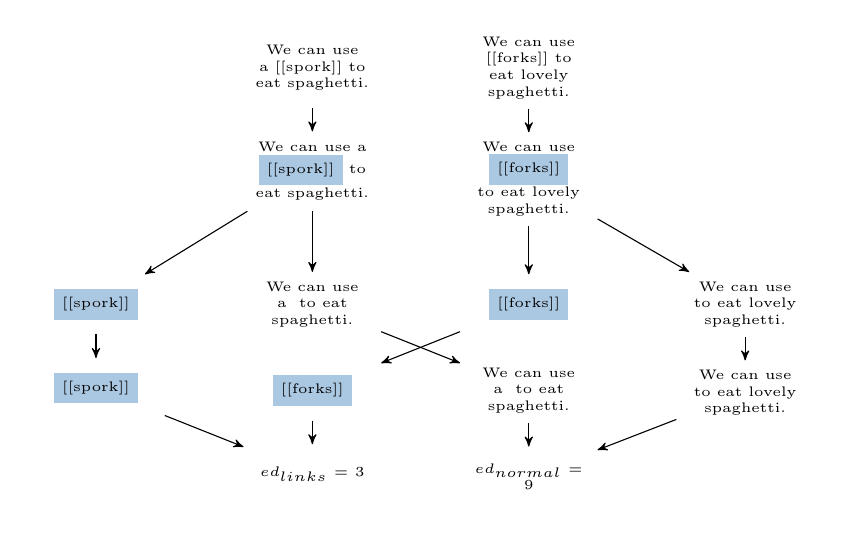
\begin{tikzpicture}[
      block1/.style={
        text width=1.5cm, 
        minimum height=1cm,
        align=center,
        anchor=north,
        font=\tiny,
      },
      block2/.style={
        text width=1.5cm, 
        minimum height=0.75cm,
        align=center,
        anchor=north,
        font=\tiny,
      }
    ]
    \node (a) [block1] {We can use a [[spork]] to eat spaghetti.};

    \node (b) [block1, right=1cm of a]{We can use [[forks]] to eat lovely
      spaghetti.};

    \node (c) [block1,below=0.3cm of a]{We can use a \hilight{[[spork]]} to eat
      spaghetti.};

    \node (d) [block1,below=0.3cm of b]{We can use \hilight{[[forks]]} to eat lovely
      spaghetti.};

    \node (e) [block2,below left=0.8cm and 1cm of c] {\hilight{[[spork]]}};
    
    \node (f) [block2,right=1cm of e] {We can use a\ \ to eat spaghetti.};

    \node (g) [block2,right=1cm of f] {\hilight{[[forks]]}};
    
    \node (h) [block2,right=1cm of g] {We can use\ \ to eat lovely spaghetti.};

    \node (i) [block2,below=0.3cm of e] {\hilight{[[spork]]}}; 
        
    \node (j) [block2,below=0.3cm of f] {\hilight{[[forks]]}}; 
    
    \node (k) [block2,below =0.3cm of g] {We can use a\ \ to eat
      spaghetti.};

    \node (l) [block2,below =0.3cm of h] {We can use\ \ to eat lovely spaghetti.};

    \node (m) [block2,below= 0.3cm of j] {$ed_{links} = 3$};

    \node (n) [block2,below =0.3cm of k] {$ed_{normal} = 9$};

    \draw [->] (a) -- (c);
    \draw [->] (b) -- (d);
    \draw [->] (c) -- (e);
    \draw [->] (c) -- (f);
    \draw [->] (d) -- (g);
    \draw [->] (d) -- (h);
    \draw [->] (e) -- (i);
    \draw [->] (g) -- (j);
    \draw [->] (f) -- (k);
    \draw [->] (h) -- (l);
    \draw [->] (i) -- (m);
    \draw [->] (j) -- (m);
    \draw [->] (k) -- (n);
    \draw [->] (l) -- (n);

  \end{tikzpicture}
  \caption{Diagram identification of link text, splitting text into
    normal and link segments, and performing separate levenshtein
    distance calculations}
\label{fig:split-diff}
\end{figure}
\end{frame}

\begin{frame}{Pair-distance calculation}{Algorithm}
  \tiny
  \begin{algorithmic}
    \State $regexes \gets $\{
    \Statex \tab`math1': `$<$math$>$((?!$<${\textbackslash}/math$>$).)*$<${\textbackslash}/math$>${\textbackslash}S',
    \Statex \tab`math2': `\{\{math((?!\}\}).)*\}\}',
    \Statex \tab`bquote': `$<$blockquote$>$((?!$<${\textbackslash}/blockquote$>$).)*$<${\textbackslash}/blockquote$>${\textbackslash}S',...
    \Statex\}\Comment{Regexes that recognise single Wikimarkup tags}
    \State $reggroups \gets $\{\label{dist-calc-groups}
    \Statex  \tab`maths':(regexes[`math1'], regexes[`math2']),...
    \Statex \}\Comment{Group of regexes by 'species'}
    \State $distances \gets \emptyset$
    \Function{PairDistance}{$str1,str2$}
    \State $strs \gets [str1, str2]$
    \ForAll {$key, reg \in reggroups$}
    \State $comparestr \gets [\emptyset , \emptyset]$
    \For {$i \gets 0,1$}
    \State $matches \gets reg.matches(strs[i])$
    \ForAll {$m \in matches$}
    \State $match, strs[i] \gets $extractsplit($m.start, m.end, strs[i]$)
    \State $comparestr[i] \gets comparestr[i] + match$
    \EndFor
    \EndFor
    \If {length($comparestr[0]$)$ > 0$ OR length($comparestr[1]$)$ > 0$}
    \State $distances[key] \gets LevDist(comparestr[0], comparestr[1])$ \label{mprocess-spawn}
    \Else
    \State $distances[key] \gets 0$
    \EndIf
    \EndFor
    \State $distances[$`$norm$'$] \gets LevDist(strs[0], strs[1])$
    \Comment{Process the remainder}
    \State return $distances$\label{mprocess-return}
    \EndFunction
  \end{algorithmic}
\end{frame}

\begin{frame}{Pair-distance calculation}{Implementation}
  \begin{itemize}
  \item C++ core
  \item Python wrapper
 \item multi-processing for the separate Levenshtein distance
    calculations
  \end{itemize}

  \onslide<2>{
    
    Though we are inevitably waiting on the final process, we still
    notice sizable increase in speed.

    \begin{figure}
      \tiny
      \centering
      \begin{tikzpicture}[x=0.25cm, y=0.25cm]
        \draw[step=.1cm,gray,very thin] (0,6) grid (30,5);
        \draw[step=.1cm,gray,very thin] (0,4) grid (30,3);
        \draw[step=.1cm,gray,very thin] (0,2) grid (30,1);
        \draw[step=.1cm,gray,very thin] (0,0) grid (30,-1);
        
        \draw[dashed, navyblue] (2,1) -- (2,0);
        \draw[dashed, navyblue] (5,3) -- (5,0);
        \draw[dashed, navyblue] (8,5) -- (8,0);
        \draw[dashed, navyblue] (10,1) -- (10,0);
        \draw[dashed, navyblue] (9,3) -- (9,0);
        \draw[dashed, navyblue] (27,5) -- (27,0);

        \draw[fill, redi] (0,0) rectangle (2,-1);
        \draw[fill, redi] (3,0) rectangle (5,-1);
        \draw[fill, redi] (6,0) rectangle (8,-1);
        
        \draw[fill, blue] (2,2) rectangle (10,1);
        \draw[fill, blue] (5,4) rectangle (9,3);
        \draw[fill, blue] (8,6) rectangle (27,5);

        \draw[fill, beige] (27,0) rectangle (30,-1);


        \draw(a)[fill, redi] (0,-2) rectangle (4,-2.5);
        \node[font=\tiny] at (5,-3) {Regex splitting operations};

        \draw(b)[fill, blue] (11,-2) rectangle (15,-2.5);
        \node[font=\tiny] at (14.7,-3) {Levenshtein calculations};

        \draw(c)[fill, beige] (22,-2) rectangle (26,-2.5);
        \node[font=\tiny] at (24.9,-3) {Database insertion};

        \node[font=\tiny, align=left] at (2,6.35) {\tiny Child process 3};
        \node[font=\tiny, align=left] at (2,4.35) {\tiny Child process 2};
        \node[font=\tiny, align=left] at (2,2.35) {\tiny Child process 1};    
        \node[font=\tiny, align=left] at (2,0.35) {\tiny Parent process};
        
      \end{tikzpicture}
    \end{figure}

  }
\end{frame}
\note{Small articles are fast, and even large articles were small
  articles once}

  \subsection{Edit and share graphs}
  \begin{frame}{Edit and Share graphs}
    We sum the weights of the rewards, group by user and normalize. We
    can compare with different weighted versions, and edit count.

    \only<1>{

      \includegraphics[width=\linewidth,height=\textheight,keepaspectratio,resolution=600]{img/lastolympianedit.png}

    }

    \only<2>{

      \includegraphics[width=\linewidth,height=\textheight,keepaspectratio,resolution=600]{img/lastolympianshare.png}

    }

    \only<3>{

      \includegraphics[width=\linewidth,height=\textheight,keepaspectratio,resolution=600]{img/zambijoedit.png}

    }

    \only<4>{

      \includegraphics[width=\linewidth,height=\textheight,keepaspectratio,resolution=600]{img/zambijoshare.png}

    }

    \only<5>{

      \includegraphics[width=\linewidth,height=\textheight,keepaspectratio,resolution=600]{img/belvoiredit.png}

    }

    \only<6>{

      \includegraphics[width=\linewidth,height=\textheight,keepaspectratio,resolution=600]{img/belvoirshare.png}

    }

    \only<7>{

      \includegraphics[width=\linewidth,height=\textheight,keepaspectratio,resolution=600]{img/agrotisedit.png}

    }

    \only<8>{

      \includegraphics[width=\linewidth,height=\textheight,keepaspectratio,resolution=600]{img/argotisshare.png}

    }

  \end{frame}

  \begin{frame}{Edit and Share graphs with weights}
    The upper graph is unweighted, the lower graph weighted
    
    \onslide<1-4>{

      \includegraphics[width=\linewidth,height=0.35\textheight,keepaspectratio,resolution=600]{img/weightings/LudvigFaddeevUnweighted.png}

    }

    \only<2>{
      {\tiny maths:}\\
      \includegraphics[width=\linewidth,height=0.35\textheight,keepaspectratio,resolution=600]{img/weightings/LudvigFaddeevMaths.png}

    }

    \only<3>{
      {\tiny files / images:}\\
      \includegraphics[width=\linewidth,height=0.35\textheight,keepaspectratio,resolution=600]{img/weightings/LudvigFaddeevfilesimages.png}

    }

    \only<4>{
      {\tiny links:}\\
      \includegraphics[width=\linewidth,height=0.35\textheight,keepaspectratio,resolution=600]{img/weightings/LudvigFaddeevLinks.png}

    }
\end{frame}

  \begin{frame}{Edit and Share graphs with weights}

    \begin{alertblock}{Edit species distribution}
      In our database of ~250,000 revisions:
      \begin{tabular}{l|r|r}
        \textbf{type} & \textbf{edit op count} & \textbf{\%}\\
        maths & 72,284 & 0.00003\%\\
        structure & 2,989,005 & 0.00109\%\\
        links  &   12,422,194 & 0.00454\%\\
        normal& 2,717,266,294 & 0.99326\%\\
        citations & 2,789,216 & 0.00102\%\\
        filesimages& 166,518 & 0.00006\%\\
      \end{tabular}
    \end{alertblock}

    \only<2>{

      Reasons?
      \begin{itemize}
      \item Wikimarkup must be learnt
      \item Using makrup is less natural
      \item Copyright problems 
        \end{itemize}
    }

  \end{frame}

  \subsection{Trajectory calculation}  
  \begin{frame}{Trajectory calculation}{History plotting}
    
    We want to augment our first measure by analysing context. Our
    steps are:
    \begin{itemize}
      \item Take the final revision
      \item Compare to every revision in turn
    \end{itemize}
    
    \onslide<2->{
      The result is a map of how close each version was to the final
      at each point in that history:
      
        \centering
        \pgfplotsset{width=0.5\textwidth}
        \begin{tikzpicture}
          \begin{axis}[
              title={\tiny Dummy revision history},
              ylabel={\tiny Ed. distance from final},
              xlabel={\tiny revision ID},
            ]
            \addplot [navyblue] table {dat/dummy_history.dat};
            \addplot [navyblue, only marks] table {dat/dummy_history.dat};
          \end{axis}
        \end{tikzpicture}
    }

  \end{frame}

  \begin{frame}{Trajectory calculation}{Use for preening}
    \centering
    \only<1>{ 
        \pgfplotsset{width=0.8\linewidth}
        \begin{tikzpicture}
          \begin{axis}[
              title={Identifying discarded work}
            ]
            \addplot [navyblue] table {dat/dummy1.dat};
            \addplot [redi] table {dat/dummy2.dat};
            \addplot [navyblue] table {dat/dummy3.dat};
            \addplot [navyblue, only marks] table {dat/dummy4.dat};
          \end{axis}
        \end{tikzpicture}
    }
    \only<2>{ 
      \pgfplotsset{width=0.8\linewidth}
      \begin{tikzpicture}
        \begin{axis}[
            title={Identifying a preening area}
          ]
          \addplot [navyblue] table {dat/dummy1.dat};
          \addplot [redi] table {dat/dummy5.dat};
          \addplot [navyblue] table {dat/dummy6.dat};
          \addplot [navyblue, only marks] table {dat/dummy4.dat};
          \fill [greeni!25,fill opacity=0.5] (axis cs:4,13) rectangle (rel axis
          cs:1,0);
          \addplot[redi,dashed,update limits=false] 
          coordinates {(-2,13) (14,13)};
          \addplot[redi,dashed,update limits=false] 
          coordinates {(4,-2) (4,23)};
        \end{axis}
      \end{tikzpicture}
    }
    \only<3>{ 
      \pgfplotsset{width=0.8\linewidth}
      \begin{tikzpicture}
        \begin{axis}[
            title={Identifying a preening area}
          ]
          \addplot [navyblue] table {dat/dummy1.dat};
          \addplot [redi] table {dat/dummy7.dat};
          \addplot [navyblue] table {dat/dummy6.dat};
          \addplot [navyblue, only marks] table {dat/dummy8.dat};
          \fill [greeni!25,fill opacity=0.5] (axis cs:4,13) rectangle (rel axis
          cs:1,0);
          \addplot[redi,dashed,update limits=false] 
          coordinates {(-2,13) (14,13)};
          \addplot[redi,dashed,update limits=false] 
          coordinates {(4,-2) (4,23)};
        \end{axis}
      \end{tikzpicture}
    }
    \only<4>{
      We finally decide not to `preen', but to grade each contribution
      according to the degree to which it caused an approach of the
      final version. 
   	}
\end{frame}

    \begin{frame}[fragile]{Trajectory calculation}{Getting greater context}

      We finally decide not to `preen', but to grade each contribution
      according to the degree to which it caused an approach of the
      final version.   
    
    \begin{figure}
      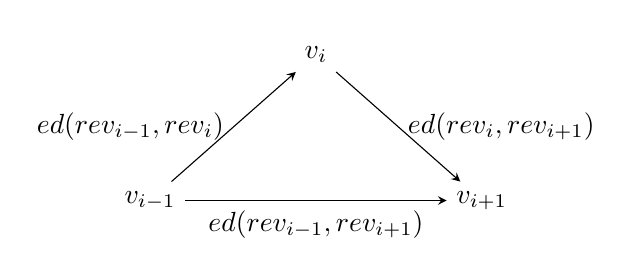
\begin{tikzpicture}
        \matrix (m) [matrix of math nodes, row sep=4em, column
          sep=4em]{ & v_i & \\ v_{i-1} & & v_{i+1}\\ };
        \path[-stealth] (m-2-1) edge node [left]
             {$ed(rev_{i-1},rev_i)$} (m-1-2) edge node [below]
             {$ed(rev_{i-1},rev_{i+1})$} (m-2-3) (m-1-2) edge node
             [right] {$ed(rev_i,rev_{i+1})$} (m-2-3); 
      \end{tikzpicture}
    \end{figure}
\end{frame}

 \begin{frame}{Trajectory calculation}{The Wikitrust software}
   Highlighted and measured the trust a reader could have in each
   word, given it's age.\cite{Adler2007}

   \begin{itemize}
   \item <1-> A culmination of a lot of existing and original work
   \item <2-> Useless \cite{Lucassen2011}
   \end{itemize}
   
   \includegraphics[width=\linewidth, height=\textheight, keepaspectratio, clip=true, resolution=600]{img/wikitrust.png}

 \end{frame}

  \begin{frame}{Trajectory calculation}{Defining gradient factor}
    \begin{figure}
      \tiny
      \centering
      \begin{subfigure}[b]{\linewidth}
        \tiny
        \centering
        \[gfactor(\Delta x,\Delta y) = \left\{ 
        \begin{array}{l l l}
          1 & \quad \text{if ${\Delta}x = 0$ and ${\Delta}y < 0$ }\\
          0 & \quad \text{if ${\Delta}x = 0$ and ${\Delta}y >= 0$ }\\
          \frac{arctan({\Delta}y/{\Delta}x)}{\pi}&\quad\text{if ${\Delta}x > 0$}
        \end{array} \right.\]
      {\tiny gradient factor definition, with $\Delta x$ as
        change in time and $\Delta y$ as difference in to-final edit
        distance}
      \end{subfigure}\\
      \vspace{4mm}
      \onslide<2>{
        \begin{subfigure}[b]{\linewidth}
          \tiny
          \centering
          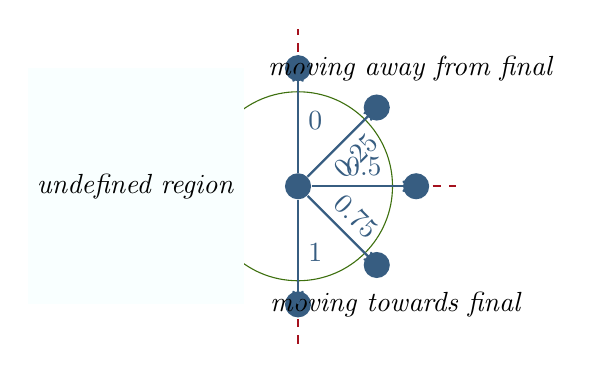
\begin{tikzpicture}[x=0.5cm,y=0.5cm]

            \draw[thick,redi,dashed] (4,0) -- (4,1);
            \draw[thick,redi,dashed] (4,7) -- (4,8);
            \draw[thick,redi,dashed] (7,4) -- (8,4);
            \draw [greeni] (4,4) circle (1.2cm);
            \node[fill,navyblue,circle] at (4,4) (o) {};
            \node[fill,navyblue,circle] at (7,4) (a) {};
            \node[fill,navyblue,circle] at (6,2) (b) {};
            \node[fill,navyblue,circle] at (6,6) (c) {};
            \node[fill,navyblue,circle] at (4,1) (d) {};
            \node[fill,navyblue,circle] at (4,7) (e) {};
            
            \node[fill=owhite,left=0.5cm of o, minimum height=3cm]{\textit{undefined region}};
            \node at (6,7) {\textit{~\ ~\ ~\ ~moving away from final}};
            \node at (6,1) {\textit{\ ~\ ~moving towards final}};
            
            \draw [thick, navyblue, ->] (o) -- (7,4) node[sloped, midway, above]{$0.5$};
            \draw [thick, navyblue, ->] (o) -- (6,2) node[sloped, midway, above]{$0.75$};
            \draw [thick, navyblue, ->] (o) -- (6,6) node[sloped, midway, below]{$0.25$};
            \draw [thick, navyblue, ->] (o) -- (4,1) node[midway, right]{$1$};
            \draw [thick, navyblue, ->] (o) -- (4,7) node[midway, right]{$0$};
          \end{tikzpicture}
          {\tiny mapping gradient factor to an arc}
        \end{subfigure}
      }
    \end{figure}
  \end{frame}
  
  \begin{frame}{Trajectory calculation}{Defining gradient factor}
      \pgfplotsset{width=0.8\linewidth}
      \begin{tikzpicture}
        \begin{axis}[
            title={`Argument history'}
          ]
          \addplot [navyblue] table {dat/dummy9.dat};
          \addplot [navyblue, only marks] table {dat/dummy9.dat};
        \end{axis}
      \end{tikzpicture}

  \end{frame}

  \begin{frame}{Trajectory calculation}{Algorithm}
      \begin{algorithmic}
        \tiny
        \Procedure{TrajectoryCalculation}{$revids, domain$}
        \State $target \gets $database.gettext($revids[-1]$)\Comment{Last revision in list is most recent}
        \For {$i \gets length(revids), 0$}
        \If{trajectory distance not already in database}
        \State $str1 \gets $database.gettext($revids[i]$)
        \State $dist \gets $LevDist($str1, target$)
        \State $database.inserttrajectoryinsert(dist)$    
        \EndIf
        \EndFor
        \For{$i \gets 0, length(revids)$}
        \State $dist2 \gets $database.gettrajectory($revids[i],domain$)
        \State $dist1 \gets$ database.gettrajectory($revid[i-1],domain$)
        \State $time2 \gets $database.gettimestamp($revid[i],domain$)
        \State $time1 \gets $
        \LineIf{database.gettimestamp($revid[i-1],domain$)}{$i \neq 0$}{$timex$} 
        \State ${\Delta}x \gets time2 - time1$
        \State ${\Delta}y \gets dist2 - dist1$
        \If{${\Delta}x > 0$}
        \State $gradient = \frac{arctan({\Delta}y/{\Delta}x)}{\pi}$ 
        \ElsIf{$x = 0$}
        \State $gradient = $\LineIf{1}{$y < 0$}{0}
        \EndIf
        \State database.insertgradient($revid[i],domain,gradient$)
        \EndFor
        \EndProcedure
      \end{algorithmic}
  \end{frame}

  \subsection{Implementation}
  \begin{frame}{Implementation}
    \begin{figure}
      \centering
      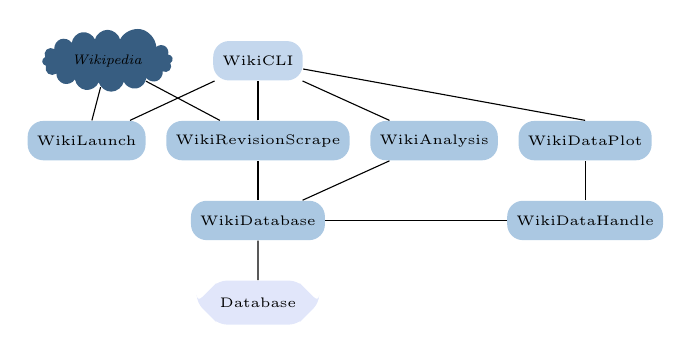
\begin{tikzpicture}[align=center,node distance=0.5cm,font=\tiny]

        \node (database)[dtb, fill=col1]{Database};

        \node (wikidata)[bx, fill=col2, above=of database]{WikiDatabase};

        \node (wikifetch)[bx, fill=col2, above=of wikidata]{WikiRevisionScrape};

        \node (wikilaunch)[bx, fill=col2, left=0.25cm of wikifetch]{WikiLaunch};

        \node (analysis)[bx, fill=col2, right=0.25 of wikifetch]{WikiAnalysis};
        
        \node (datplot)[bx, fill=col2,  right=0.25 of analysis]{WikiDataPlot};

        \node (datahandle)[bx, fill=col2, below= of datplot]{WikiDataHandle};

        \node (wikicli)[bx, fill=col5, above=of wikifetch]{WikiCLI}; 
        
        \node (wikipedia)[cld, fill=col4, left=of wikicli]{\textit{Wikipedia}};

        \draw [-] (database) -- (wikidata); 

        \draw [-] (wikidata) -- (analysis); 

        \draw [-] (wikidata) -- (wikifetch); 

        \draw [-] (wikidata) -- (datahandle); 

        \draw [-] (wikifetch) -- (wikipedia); 

        \draw [-] (wikilaunch) -- (wikipedia); 

        \draw [-] (datahandle) -- (datplot);

        \draw [-] (datplot.north) -- (wikicli); 

        \draw [-] (wikifetch) -- (wikicli); 

        \draw [-] (wikicli) -- (analysis); 

        \draw [-] (wikicli) -- (wikilaunch);      

      \end{tikzpicture}
      \caption{Diagram showing the connections between entities in python implementation}
    \end{figure}
\end{frame}

%% \begin{frame}
%%   \frametitle{Alignment problems}
%%   Later we would wonder if we could afford to do away with the
%%   trajectory calculations.
%% \end{frame}

  %%%%%%%%%%%%%%%%%%%%%%%%%%%%%%%%%%%%%%%%%%%%%%%%%%
  %%%%%%%%%%%%%%%%%%%%%%%%%%%%%%%%%%%%%%%%%%%%%%%%%%
  %%%%% 
  %%%%% OUR FINDINGS
  %%%%%
  %%%%%%%%%%%%%%%%%%%%%%%%%%%%%%%%%%%%%%%%%%%%%%%%%%
  %%%%%%%%%%%%%%%%%%%%%%%%%%%%%%%%%%%%%%%%%%%%%%%%%%
\subsection{Plotting with trajectory}
  \begin{frame}{Edit and Share graphs with gradient factor}
    The lower graph includes the gradient factor.

    \only<1>{
      \small{unweighted:}\\
      \includegraphics[width=\linewidth,height=0.35\textheight,keepaspectratio,resolution=600]{img/weightings/LudvigFaddeevUnweighted.png}
      
      \includegraphics[width=\linewidth,height=0.35\textheight,keepaspectratio,resolution=600]{img/weightings/LudvigFaddeevUnweightedGradient.png}
    }

    \only<2>{
      \small{maths:}\\
      \includegraphics[width=\linewidth,height=0.35\textheight,keepaspectratio,resolution=600]{img/weightings/LudvigFaddeevMaths.png}
      
      \includegraphics[width=\linewidth,height=0.35\textheight,keepaspectratio,resolution=600]{img/weightings/LudvigFaddeevMathsGradient.png}
    }

    \only<3>{
      \small{links:}\\
      \includegraphics[width=\linewidth,height=0.35\textheight,keepaspectratio,resolution=600]{img/weightings/LudvigFaddeevLinks.png}
      
      \includegraphics[width=\linewidth,height=0.35\textheight,keepaspectratio,resolution=600]{img/weightings/LudvigFaddeevLinksGradient.png}
    }
  \end{frame}


  \begin{frame}{Typical trajectory graphs}

    \only<1>{

      \includegraphics[width=\linewidth,height=\textheight,keepaspectratio,resolution=600]{img/altman.png}

    }

    \only<2>{

      \includegraphics[width=\linewidth,height=\textheight,keepaspectratio,resolution=600]{img/silver.png}

    }

    \only<3>{

      \includegraphics[width=\linewidth,height=\textheight,keepaspectratio,resolution=600]{img/utica.png}

    }

    \only<4>{

      \includegraphics[width=\linewidth,height=\textheight,keepaspectratio,resolution=600]{img/basketball.png}

    }


    \only<5>{

      \includegraphics[width=\linewidth,height=\textheight,keepaspectratio,resolution=600]{img/kelly.png}

    }    

    \only<6>{

      \includegraphics[width=\linewidth,height=\textheight,keepaspectratio,resolution=600]{img/pl291709traj.png}

    }    

  \end{frame}

  \begin{frame}{Small Wikipedia graphs}
    ...showing evidence of bot link migration

    \only<1>{

      \includegraphics[width=\linewidth,height=\textheight,keepaspectratio,resolution=600]{img/marroko.png}

    }


    \only<2>{

      \includegraphics[width=\linewidth,height=\textheight,keepaspectratio,resolution=600]{img/sicilia.png}

    }

    \only<3>{

      \includegraphics[width=\linewidth,height=\textheight,keepaspectratio,resolution=600]{img/icnahi.png}

    }

    \only<4>{

      \includegraphics[width=\linewidth,height=\textheight,keepaspectratio,resolution=600]{img/957.png}

    }

    \only<5>{

      \includegraphics[width=\linewidth,height=\textheight,keepaspectratio,resolution=600]{img/hif1042.png}

    }

    \only<6>{

      \includegraphics[width=\linewidth,height=\textheight,keepaspectratio,resolution=600]{img/fo1937.png}

    }

  \end{frame}

  \begin{frame}{Combination plots}

    \only<1>{

      \includegraphics[width=\linewidth,height=\textheight,keepaspectratio,resolution=600]{img/specialcombo/en5800180.png}

    }

    \only<2>{

      \includegraphics[width=\linewidth,height=\textheight,keepaspectratio,resolution=600]{img/specialcombo/en4834368.png}

    }
    
    \only<3>{

      \includegraphics[width=\linewidth,height=\textheight,keepaspectratio,resolution=600]{img/specialcombo/en21113485.png}

    }
    
    \only<4>{

      \includegraphics[width=\linewidth,height=\textheight,keepaspectratio,resolution=600]{img/specialcombo/en2387806.png}

    }
    
    \only<5>{

      \includegraphics[width=\linewidth,height=\textheight,keepaspectratio,resolution=600]{img/specialcombo/sheldrake.png}

    }

    \only<6>{

      \includegraphics[width=\linewidth,height=\textheight,keepaspectratio,resolution=600]{img/dereksmartcombo.png}

    }
  \end{frame}

  \section{Evaluation}
  \begin{frame}{Alignment of levenshtein distance}
    \only<1>{

      Is it possible to do away with the weights, and get an idea of
      the distance between each pair using the trajectory diagram?

      Deleting some text and reinserting over two operations may by
      less efficient than swapping in one.

      But our splitting of the text causes further problems:
      
      {\tiny $ed($``We can use a [[spork]] to eat spaghetti.''$,$``We can use forks
      to eat lovely spaghetti.''$) = 7$}
      
    }

    \only<2>{
      
    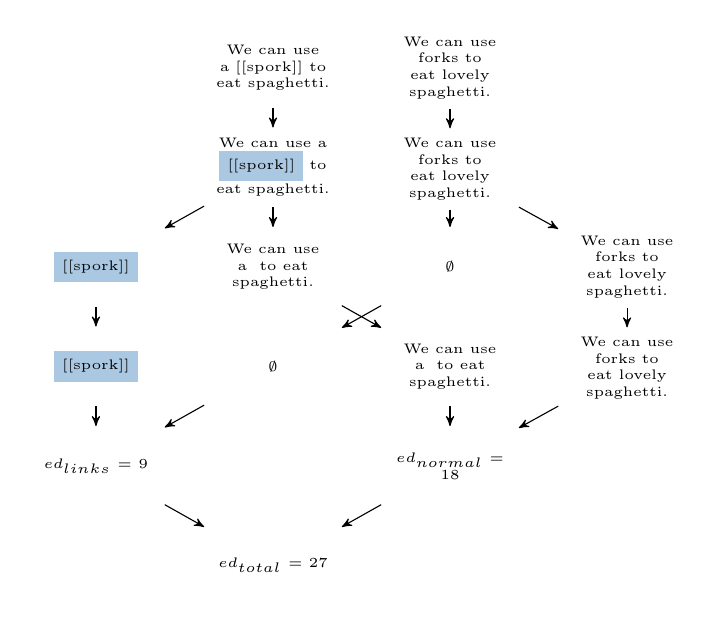
\begin{tikzpicture}[
        block1/.style={
          text width=1.5cm, 
          minimum height=1cm,
          align=center,
          anchor=north,
          font=\tiny
        },
        block2/.style={
          text width=1.5cm, 
          minimum height=1cm,
          align=center,
          anchor=north,
          font=\tiny
        },
        font=\small
      ]
      \node (a) [block1] {We can use a [[spork]] to eat spaghetti.};

      \node (b) [block1, right=0.5 of a]{We can use forks to eat lovely
        spaghetti.};

      \node (c) [block1,below=0.25 of a]{We can use a \hilight{[[spork]]} to eat
        spaghetti.};

      \node (d) [block1,below=0.25 of b]{We can use forks to eat lovely
        spaghetti.};

      \node (e) [block2,below left=0.25cm and 0.5cm of c] {\hilight{[[spork]]}};
      
      \node (f) [block2,right=0.5 of e] {We can use a\ \  to eat spaghetti.};

      \node (g) [block2,right=0.5 of f] {$\emptyset$};
      
      \node (h) [block2,right=0.5 of g] {We can use forks to eat lovely
        spaghetti.};

      \node (i) [block2,below=0.25 of e] {\hilight{[[spork]]}}; 
      
      \node (j) [block2,below=0.25 of f] {$\emptyset$}; 
      
      \node (k) [block2,below =0.25 of g] {We can use a\ \  to eat
        spaghetti.};

      \node (l) [block2,below =0.25 of h] {We can use forks to eat lovely
        spaghetti.};

      \node (m) [block2,below= 0.25 of i] {$ed_{links} = 9$};

      \node (n) [block2,below =0.25 of k] {$ed_{normal} = 18$};
      
      \node (o) [block2,below left=0.25cm and 0.5cm of n] {$ed_{total} = 27$};

      \draw [->] (a) -- (c);
      \draw [->] (b) -- (d);
      \draw [->] (c) -- (e);
      \draw [->] (c) -- (f);
      \draw [->] (d) -- (g);
      \draw [->] (d) -- (h);
      \draw [->] (e) -- (i);
      \draw [->] (g) -- (j);
      \draw [->] (f) -- (k);
      \draw [->] (h) -- (l);
      \draw [->] (i) -- (m);
      \draw [->] (j) -- (m);
      \draw [->] (k) -- (n);
      \draw [->] (l) -- (n);
      \draw [->] (m) -- (o);
      \draw [->] (n) -- (o);

    \end{tikzpicture}
 
    Diagram from work leading up to the Wikitrust Software
 }

\end{frame}

\begin{frame}{Other optimisations}

  \begin{description}
    \item[\textbf{Identify moves of large blocks of text}] structure
      of Wikipedia article can be weak.\cite{Giles2005}
    \item[\textbf{Refinement of gradient factor}] If someone makes two
      consecutive edits, is the reward less than or greater than if
      they made the edit in one go?
    \item[\textbf{Better data}] Wikipedia dumps...
    \item[\textbf{Further subjects}] Source control...
  \end{description}
  
  \only<2>{

     \includegraphics[width=\linewidth,height=0.4\textheight,keepaspectratio,resolution=600]{img/myproject101.png}

  }
  
\end{frame}

\begin{frame}{Machine learning validation of gradient factor}
  We wanted to see if we could predict gradient factor using other
  weights, size, etc.

  If we can predict gradient factor, we can see if some of the things
  we analysed come to bear on how much that edit will affect the final
  form.
 
  \onslide<2->{

    We tried regression and classification techniques, without much
    success. 
  }

\onslide<3->{
  Not enough information
  \begin{itemize}
    \item More information about text?
    \item More information about context?
  \end{itemize}
}
\end{frame}

\section{Conclusions}
\begin{frame}{Conclusions}

\begin{enumerate}[<+->]  
\item If we are distributing royalties to collaborators, then we must also consider the item has worth in its current form.
\item If we have a full history, we can trace the provenance of the parts of the current form.
\item We can't assume that edits that aren't (partially) present at the end aren't important to the shape and nature of the current form.
\item Qualitative analysis of the fact of each edit is misguided.
\item More important is the work's `path', and the discussions around
  it. (Easily accessible usually but perhaps not in programming.)
\end{enumerate}
\end{frame}

  \section{References}
  \begin{frame}[allowframebreaks] %allow to expand references to multiple frames (slides)
    \frametitle{References}
    \scriptsize{\bibliographystyle{plain}}
    \bibliography{presentation} %bibtex file name without .bib extension
  \end{frame}

\end{document}
